\chapter{NeSC Architecture}
\label{chap:architecture}


%%%%%%%%%%%%%%%%%%%%
\begin{figure*}[ht]
  %% \vspace*{-1.5ex}
  \centering
  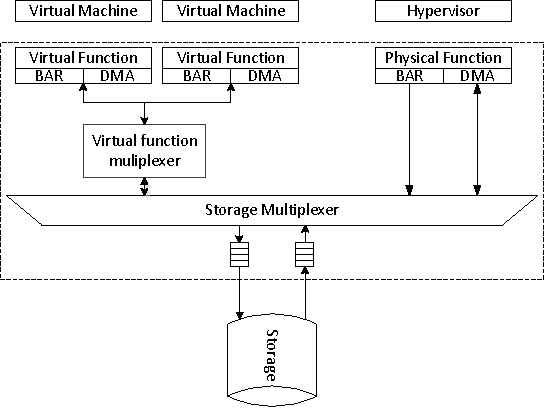
\includegraphics[width=1\columnwidth]{figs/architecture.pdf}
  \caption{An outline of the NeSC architecture. The PF and VFs each have a set of control registers and request/response queues. The core NeSC microarchitecture multiplexes the activity of the individual VFs.}
  \label{fig:architecture}
\end{figure*}
%%%%%%%%%%%%%%%%%%%%

% Add table of the virtual function interface.


% registers only hypervisor can access:
% bus address of extent tree root
% requested write address and size for hypervisor to read when updating tree
%
%registers accessed by virtual machine driver
%lba - start address for upcoming sg list.
%write command list
%read command list
%dma status


%% \section{NeSC PCIe Interface}
%% \label{arch:interface}
%% \comment{change name of this section}

As an SR-IOV device, NeSC presents itself as multiple devices on the PCIe interconnect. The architecture must maintain a separate context for each PCIe device (PF and VFs), but a key tenet of the microarchitecture is multiplexing traffic from the different devices.

Figure~\ref{fig:architecture} outlines the core design of the NeSC architecture. For each function (PF and VF alike), NeSC maintains a set of  control registers and request/response queues. All requests sent to the
different functions are multiplexed through the address translation and request service units. Similarly, all traffic between the host and the device is multiplexed through a single DMA engine. 

\section{PCIe Interface}
\label{arch:pcie}

\subsection*{PCIe Transactions}
\label{subsec:tlp}
The PCIe interconnect is based on point-to-point topology, with separate serial links connecting every device to the root complex (host).
Communication between devices to themselves, and between devices to the root complex is done by sending and receiving PCIe requests (configuration, I/O or memory read/write). These requests form a \emph{Transactional Layer
  Packet} (TLP) and carry the request info (type, address, size etc.). Whenever the CPU accesses the device's address space, a TLP is generated and sent by the root complex to NeSC.  
Every request received by the NeSC device is labeled with the ID of the NeSC function to which it was sent. This enables the multiplexed facilities to associate requests with a specific function (according to the SR-IOV specification, the ID of the PF is 0). PCIe addressing is hierarchical, and each entity on the interconnect is identified by a triplet: the PCIe \emph{bus ID}, the ID of the device on the bus (\emph{device ID}), and the function inside the device (\emph{function ID}). In PCIe parlance, addresses are referred to as \emph{bus:device:function} triplets or \emph{BDF} for short. Since PCIe addresses of the different NeSC functions share the same bus and device IDs, associating each request with its originating function ID is sufficient for accurate bookkeeping.
The BDF triplet is originated by the PCIe root complex and is unforgeable by a virtual machine. The VM has access only to a specific VF, therefore the request generated by the root complex  will contain the BDF concurrent to that VF.     

\subsection*{Configuration Space}
PCIe devices have a set of registers referred to as configuration space. Configuration space registers are mapped to memory locations. Device drivers must have access to the configuration space, and operating systems typically use APIs to allow access to device configuration space.
Communication with a PCIe device is handled through \emph{base address registers} (BARs). BARs have a predetermined size, and are mapped to the system's logical address space when the PCIe interconnect is scanned (typically by the system's firmware). Since each BAR is assigned a logical bus address, the hypervisor can map the BARs directly to clients' virtual address space, and to its own.

Although NeSC assigns a BAR for each function (physical and virtual alike), the control registers for all functions can be mapped to a single physical structure inside the device.
The PCIe specifications make it possible to define control registers as offsets into a device's BAR. When a certain offset inside a BAR is read from or written to, the PCIe device internally translates the offset to an address in a shared structure.
Since our prototype can support up to 64 VFs (and the additional PF), the NeSC prototype uses a single 130KB SRAM array (2048B per function).

The set of VF-specific control registers are listed as follows (the PCIe specification mandates a number of additional standard control registers, omitted for brevity).
\begin{enumerate}
\item
  \textbf{DMAListEntry} (8B) \quad
  This register is where the driver writes the nodes of a scatter-gather list. Each node that is written here
  is immediately appended to a list NeSC maintains and a new node can override the old value. The driver sends the scatter-gather list to NeSC by writing all the nodes to this register one by one.

\item
  \textbf{ExtentTreeRoot} (8B)\quad
  This register contains the base address (in host memory) of the root node of the extent tree associated with a VF. It is set by the hypervisor when a new VF is created. 
%
\item
  \textbf{MissAddress, MissSize} (8B, 4B)\quad
  These two registers are set by NeSC when a translation of a write request sent to the VF misses in the extent tree. After setting these values, NeSC sends an interrupt to the hypervisor so it will allocate additional physical space to the file associated with the VF.
%
\item
  \textbf{RewalkTree} (4B)\quad
  This register is used by the hypervisor to signal NeSC that the physical storage allocation has succeeded. When the hypervisor writes a value of 1 to a VF's RewalkTree register, NeSC reissues the stalled write requests to the extent tree walk unit.
\end{enumerate}

In addition to the NeSC-specific control registers listed above, each VF also exposes a set of registers for controlling a DMA ring buffer~\cite{love10lkd}, which is the de facto standard for communicating with devices. We omit those for brevity.


\section{Kernel Drivers}
\label{arch:drivers}
As mentioned in \ref{iovirt:driver}, a device driver communicates with the NeSC device through the PCIe interconnect.
When the block layer decides to commit read/write requests to the underlying storage, it sends the requests to
the driver in the form of bio structures. The driver will translate the request to NeSC read/write requests and
return when the request is full filed.

NeSC is controlled by two device drivers, one is used by the hypervisor to access the PF, and one is used by
virtual machines to access the VF. 

\subsection*{The VF Driver}
\label{arch:vfdriver}
A VM that wants to access the NeSC device, installs the NeSC VF device driver.
When a request is sent to the driver by the block layer, the driver will map the request to a
\emph{scatter-gather} list and send the nodes to NeSC one by one. The nodes in the list are DMA requests for NeSC to execute. Each node in the list consists of:
\begin{itemize}
\item \emph{dma address}\quad
  The bus address of the current request. NeSC will DMA to/from this address.  
\item \emph{offset} \quad
  The offset from the beginining of the bus address.
\item \emph{length} \quad
  The amount of bytes to transfer. Each node is limited to represent up to 4K bytes which is exactly the size of
  a page on the system.
\end{itemize}

while sending the list, NeSC will start executing the requests one by one and when its done, NeSC will send a finished interrupt to the driver.

\subsection*{PF Driver}
\label{arch:pfdriver}
The PF driver's interface with the block layer is the same as the VF, and through it the hypervisor installs the root filesystem on NeSC.
The hypervisor uses the PF driver to manage SR-IOV capabilities. Through the driver the hypervisor creates, deletes and manages VFs. When a new VF is created, the PF driver is responsible of assigning the ExtentTreeRoot register to point to the correct base address of the extent tree.

During NeSC operation, if a VF tries to write to an unassigned block (as seen in \ref{des:write}), an interrupt will be sent by NeSC and will be handled in the PF driver. The driver will allocate and assign new blocks to the
VF extent tree and signal the VF to continue with the write request.

%%%%%%%%%%%%%%%%%%%%%%%%%%%%%%%%%%%%%%%%%%%%%%%%%%
\section{The NeSC virtual function multiplexer}
%%%%%%%%%%%%%%%%%%%%%%%%%%%%%%%%%%%%%%%%%%%%%%%%%%

%%%%%%%%%%%%%%%%%%%%
\begin{figure*}[t]
  \centering
  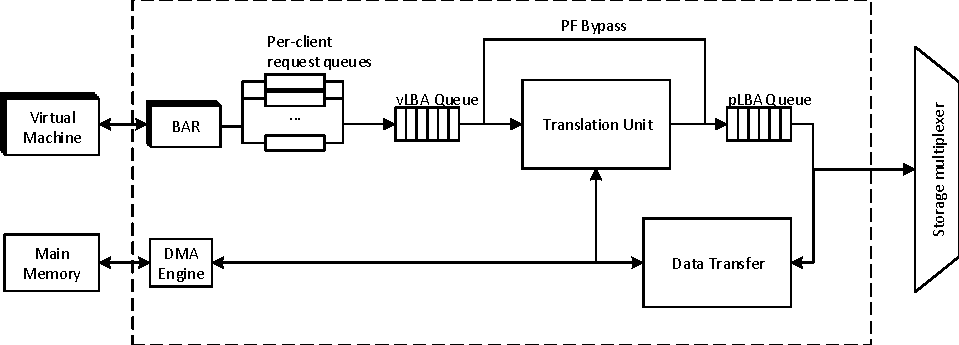
\includegraphics[width=\textwidth]{figs/virtual_function.pdf}
  \caption{High-level view of the NeSC virtual function multiplexer design. The microarchitecture multiplexes requests from the different virtual functions.}
   \label{fig:virtualfunction}
%\end{figure*}
%%%%%%%%%%%%%%%%%%%%

   \vspace*{3ex}
   
%%%%%%%%%%%%%%%%%%%%
%\begin{figure*}[t]
  \centering
  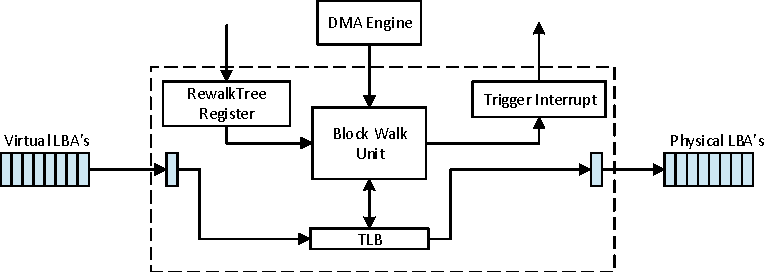
\includegraphics[width=1.1\textwidth]{figs/translation_unit.pdf}
  \caption{The vLBA-to-pLBA translation unit.}
   \label{fig:translation_unit}
\end{figure*}
%%%%%%%%%%%%%%%%%%%%

In this section we describe the implementation of the NeSC virtual function multiplexer, which is depicted in Figure~\ref{fig:virtualfunction}. The main role of the  virtual function multiplexer is to process access requests from the multiple VFs, translate their addresses to physical storage blocks, and respond to the client VM.
%
Access requests are sent by the VM's block driver. The driver typically breaks large requests into a sequence of smaller 4KB requests that match the system's page size. Requests sent from different client VMs are stored in per-client request queues. NeSC dequeues client requests in a round-robin manner in order to prevent client starvation (a full study of client scheduling algorithms and different quality-of-service guarantees is beyond the scope of this paper).

Client requests address their target storage blocks using vLBAs, or logical block addresses as viewed by the virtual device. These addresses must be translated to pLBAs using the per-VF extent tree. The client requests are therefore pushed to a shared vLBA queue for translation, along with the root pointer to their VF's extent tree.

NeSC includes a dedicated \emph{translation unit} (discussed below) that dequeues pending requests from the vLBA queue, translates their vLBAs to pLBAs and pushes the translated requests to a pLBA queue. A \emph{data transfer} unit then manages direct accesses to the persistent storage device. For write requests, the data transfer unit simply writes the data to storage and generates an acknowledge response message that will be sent to the client. For read requests, the data transfer unit reads the target data from the physical storage and prepares a response message. The message is then DMAed to the client VM's destination buffer in host memory.

While we only discuss the processing of client VM requests, NeSC also includes a dedicated out-of-band (OOB) channel to process hypervisor requests sent through the PF. The OOB channel is needed so that VF write requests whose translation is blocked will not block PF requests. The addition of the OOB is, however, simple since PF requests use pLBAs and need not be translated. The OOB channel, therefore, bypasses the NeSC flow preceding the pLBA queue and does not affect the the address translation unit.

%%%%%%%%%%%%%%%%%%%%%%%%%%%%%%%%%%%%%%%%%%%%%%%%%%
\subsection*{The vLBA-to-pLBA translation unit}
%%%%%%%%%%%%%%%%%%%%%%%%%%%%%%%%%%%%%%%%%%%%%%%%%%

The translation unit translates the vLBA addresses used in client VM requests to pLBA addresses, which can be used to access the physical storage. The translation uses the extent tree associated with a request's originating VF.

Figure~\ref{fig:translation_unit} illustrates the translation unit and its components. These include a \emph{block walk unit} that traverses the extent tree and a \emph{block translation lookaside buffer} (BTLB) that caches recent vLBA mappings. Furthermore, the unit may send interrupts to the hypervisor when a mapping is not found (e.g., when a client VM writes to an unallocated portion of its virtual device), and it is charged with observing the VF's \emph{RewalkTree} registers through which the hypervisor signals that the mapping was fixed and the extent tree can be re-examined.

%%%%%%%%%%%%%%%%%%%%
\subsubsection*{Block walk unit}
%%%%%%%%%%%%%%%%%%%%
This unit executes the block walk procedure by traversing the extent tree.
When a client VM request arrives at the unit, the root node of the associated extent tree is DMAed and the unit tries to match the vLBA to the offsets listed in the root node's entries (be they node pointers or extent pointers). The matched entry is used as the next node in the traversal, and the process continues recursively until an extent is matched. For read operations, an unmatched vLBA means that the client VM is trying to read from an unmapped file offset (a hole in the file) and zeros must be returned. If a match is not found on a write operation, the unit sets the VF's \emph{MissAddress} and \emph{MissSize} control registers, interrupts the host, and waits until the hypervisor signals that the missing blocks were allocated (using the \emph{RewalkTree} control register).

The block walk unit is designed for throughput. Since the main performance bottleneck of the unit is the DMA transaction of the next level in the tree, the unit can overlap two translation processes to (almost) hide the DMA latency.

%%%%%%%%%%%%%%%%%%%%
\subsubsection*{Block translation lookaside buffer (BTLB)}
%%%%%%%%%%%%%%%%%%%%
Given that storage access exhibits spatial locality, and  extents typically span more than one block, the translation unit maintains a small cache of the last 8 extents used in translation. Specifically, this enables the BTLB to maintain at least the last mapping for each of the last 8 VFs it serviced.

Before the translation unit begins the block walk, it checks the BTLB to see whether the currently translated vLBA matches one of the extents in the BTLB. If a match is found, the unit skips the block walk and creates a new pLBA for the output queue.
On a miss, the vLBA will be passes to the block walk unit and, after the translation completes, the mapping will be inserted to the BTLB (evicting the oldest entry).

Finally, the BTLB cache must not prevent the hypervisor from executing traditional storage optimizations (e.g., block deduplication). Consequently, NeSC enables the PF (representing the hypervisor) to flush the BTLB cache in order to preserve meta-data consistency.

\hide{
%%%%%%%%%%%%%%%%%%%%
\subsubsection*{Data Transfer unit}
%%%%%%%%%%%%%%%%%%%%
This unit interacts with the DMA engine to DMA blocks of storage to and from the storage device.

When a read command is requested by the VM, data blocks are returned by the storage multiplexer to this unit, which in turn will DMA them to the correct address according to the scatter-gather list.

When a write command is requested by the VM, the unit will DMA the blocks from memory and send packets containing the PLBA and the data to the storage multiplexer.
}

In summary, the NeSC implementation effectively balances the need to multiplex different VFs with the application of traditional optimizations such as caching and latency hiding. The following sections describe our evaluation of the proposed NeSC design.
